\documentclass[11pt,a4paper]{article}
\usepackage[utf8]{inputenc}
\usepackage[T1]{fontenc}
\usepackage[french]{babel}
\usepackage{graphicx}
\usepackage{amsmath}
\usepackage{booktabs}
\usepackage{geometry}
\usepackage{hyperref}
\geometry{margin=2.5cm}

% Inclusion des résultats calculés automatiquement par simulations/main.py
\IfFileExists{simulations/results.tex}{%
    % ======================================================================
% FICHIER GÉNÉRÉ AUTOMATIQUEMENT PAR simulations/main.py
% Ne pas modifier manuellement. Relancer 'python simulations/main.py'
% ======================================================================

% --- Cuisine ---
\newcommand{\ValTCafetiere}{1.33}
\newcommand{\ValECafetiere}{1000}
\newcommand{\ValECafetiereVeille}{1022.7}
\newcommand{\ValTBouilloire}{0.379}
\newcommand{\ValEBouilloire}{758.3}
\newcommand{\ValTMicroOndes}{0.17}
\newcommand{\ValEMicroOndes}{116.7}
\newcommand{\ValTTaque}{1.33}
\newcommand{\ValETaque}{2700.7}
\newcommand{\ValTBoiler}{1.0}
\newcommand{\ValEBoiler}{140}
\newcommand{\ValECuisineTotal}{4738.3}
\newcommand{\ValECuisineTotalKWh}{1191.1}

% --- Éclairage ---
\newcommand{\ValPLED}{1200}
\newcommand{\ValELED}{9600}
\newcommand{\ValPFluo}{420}
\newcommand{\ValEFluo}{3360}
\newcommand{\ValEEclairageTotal}{12960.0}

% --- Auxiliaires Totaux ---
\newcommand{\ValETotalAuxWh}{17698.3}
\newcommand{\ValETotalAuxKWh}{17.70}
\newcommand{\ValETotalAuxAnKWh}{4431.1}

% --- Machines d'atelier ---
% Scie à panneaux
\newcommand{\ValPnscieapanneaux}{2900}
\newcommand{\ValCosPhiscieapanneaux}{0.83}
\newcommand{\ValEtascieapanneaux}{0.84}
\newcommand{\ValChargescieapanneaux}{75}
\newcommand{\ValDureescieapanneaux}{1.00}
\newcommand{\ValPabsscieapanneaux}{2589.3}
\newcommand{\ValQscieapanneaux}{1740.0}
\newcommand{\ValIscieapanneaux}{4.50}
\newcommand{\ValEDayscieapanneaux}{2589.3}
\newcommand{\ValEYearscieapanneaux}{647.3}
% Scie radiale
\newcommand{\ValPnscieradiale}{3000}
\newcommand{\ValCosPhiscieradiale}{0.84}
\newcommand{\ValEtascieradiale}{0.85}
\newcommand{\ValChargescieradiale}{50}
\newcommand{\ValDureescieradiale}{3.00}
\newcommand{\ValPabsscieradiale}{1764.7}
\newcommand{\ValQscieradiale}{1139.9}
\newcommand{\ValIscieradiale}{3.03}
\newcommand{\ValEDayscieradiale}{5294.1}
\newcommand{\ValEYearscieradiale}{1323.5}
% Aspiration centralisée
\newcommand{\ValPnaspirationcentralisee}{3000}
\newcommand{\ValCosPhiaspirationcentralisee}{0.85}
\newcommand{\ValEtaaspirationcentralisee}{0.86}
\newcommand{\ValChargeaspirationcentralisee}{100}
\newcommand{\ValDureeaspirationcentralisee}{1.50}
\newcommand{\ValPabsaspirationcentralisee}{3488.4}
\newcommand{\ValQaspirationcentralisee}{2161.9}
\newcommand{\ValIaspirationcentralisee}{5.92}
\newcommand{\ValEDayaspirationcentralisee}{5232.6}
\newcommand{\ValEYearaspirationcentralisee}{1308.1}
% Scie sur table
\newcommand{\ValPnsciesurtable}{2800}
\newcommand{\ValCosPhisciesurtable}{0.82}
\newcommand{\ValEtasciesurtable}{0.84}
\newcommand{\ValChargesciesurtable}{50}
\newcommand{\ValDureesciesurtable}{3.00}
\newcommand{\ValPabssciesurtable}{1666.7}
\newcommand{\ValQsciesurtable}{1163.3}
\newcommand{\ValIsciesurtable}{2.93}
\newcommand{\ValEDaysciesurtable}{5000.0}
\newcommand{\ValEYearsciesurtable}{1250.0}
% Ponceuse à bande
\newcommand{\ValPnponceuseabande}{750}
\newcommand{\ValCosPhiponceuseabande}{0.80}
\newcommand{\ValEtaponceuseabande}{0.80}
\newcommand{\ValChargeponceuseabande}{100}
\newcommand{\ValDureeponceuseabande}{0.33}
\newcommand{\ValPabsponceuseabande}{937.5}
\newcommand{\ValQponceuseabande}{703.1}
\newcommand{\ValIponceuseabande}{5.10}
\newcommand{\ValEDayponceuseabande}{312.5}
\newcommand{\ValEYearponceuseabande}{78.1}
% Scie à ruban
\newcommand{\ValPnsciearuban}{1500}
\newcommand{\ValCosPhisciearuban}{0.81}
\newcommand{\ValEtasciearuban}{0.83}
\newcommand{\ValChargesciearuban}{75}
\newcommand{\ValDureesciearuban}{3.00}
\newcommand{\ValPabssciearuban}{1355.4}
\newcommand{\ValQsciearuban}{981.3}
\newcommand{\ValIsciearuban}{2.42}
\newcommand{\ValEDaysciearuban}{4066.3}
\newcommand{\ValEYearsciearuban}{1016.6}
\newcommand{\ValPabsAtelierTotal}{11802.0}
\newcommand{\ValQAtelierTotal}{7889.6}
\newcommand{\ValSAtelierTotal}{14196.2}
\newcommand{\ValCosPhiAtelier}{0.83}
\newcommand{\ValEAtelierDay}{22494.7}
\newcommand{\ValEAtelierYear}{5623.7}

% --- Bornes VE ---
\newcommand{\ValEVeAnWh}{7200000}
\newcommand{\ValEVeAnKWh}{7200}
\newcommand{\ValEVeDayWh}{28800}

% --- Consommation globale annuelle ---
\newcommand{\ValETotalAnKWh}{17254.8}
\newcommand{\ValETotalAnMWh}{17.25}
\newcommand{\ValETotalJourKWh}{68.99}

% --- Dimensionnement Raccordement ---
\newcommand{\ValPInstalledKW}{30.0}
\newcommand{\ValSInstalledKVA}{31.9}
\newcommand{\ValIMaxTotalA}{46.1}
\newcommand{\ValSSouscriteKVA}{31.9}
\newcommand{\ValISouscritA}{46.1}

% --- Photovoltaïque ---
\newcommand{\ValSolarTargetKWh}{5751.6}
\newcommand{\ValSolarRequiredKWc}{5.75}
\newcommand{\ValSolarPanelCount}{11}
\newcommand{\ValSolarActualKWc}{5.88}
\newcommand{\ValSolarActualProdKWh}{5885.0}
\newcommand{\ValSolarSurfaceMdeux}{28.4}

% --- Courant déformé mesuré ---
\newcommand{\ValCourantNPoints}{423}
\newcommand{\ValCourantIrms}{33.66}
\newcommand{\ValCourantImax}{47.46}
\newcommand{\ValCourantImin}{-47.10}
%
}

\title{\textbf{Projet UE12 : Électricité Appliquée}\\Dimensionnement de la menuiserie \og L'Électron d'Arbre \fg\\(Groupe 25)}
\author{Pierre Sluse}
\date{Année académique 2026--2027}

\begin{document}

\maketitle

\section{Introduction}
Ce rapport présente l'étude technique et le dimensionnement électrique complet de la menuiserie \og L'Électron d'Arbre \fg\ (Groupe 25). 
L'ensemble des paramètres techniques des machines, des puissances absorbées, des consommations journalières et annuelles, ainsi que le dimensionnement de l'installation photovoltaïque et du raccordement sont automatisés via un script Python orienté objet (\texttt{simulations/data.py} et \texttt{simulations/main.py}).

\section{Charges Auxiliaires (Cuisine et Éclairage)}
Afin de dimensionner le circuit électrique auxiliaire, les durées et puissances ont été converties en grandeurs énergétiques journalières et annuelles (base de 250 jours ouvrés par an).

\subsection{Cuisine}
\begin{itemize}
    \item \textbf{Cafetière} : Puissance de fonctionnement de 750\,W et veille permanente de 1\,W. À raison de 40 cafés par jour (2\,min par tasse), le temps de fonctionnement est de $\frac{40 \times 2}{60} = \ValTCafetiere$\,h/jour.
    Consommation en travail : $750 \times \ValTCafetiere = \ValECafetiere$\,Wh/jour. En intégrant la veille continue sur 24\,h, la consommation journalière totale est de \textbf{\ValECafetiereVeille\,Wh/jour}.
    \item \textbf{Bouilloire} : Puissance de 2000\,W. Pour 7 litres d'eau à 3,25\,min/L, soit une durée journalière de $\ValTBouilloire$\,h :
    Consommation : $2000 \times \ValTBouilloire = \textbf{\ValEBouilloire\,Wh/jour}$.
    \item \textbf{Micro-ondes} : Puissance de 700\,W utilisé pendant 10 minutes ($\ValTMicroOndes$\,h/jour) :
    Consommation : $700 \times \ValTMicroOndes = \textbf{\ValEMicroOndes\,Wh/jour}$.
    \item \textbf{Taque électrique} : Puissance de 2000\,W pendant 80 minutes ($\ValTTaque$\,h/jour) :
    Consommation : $2000 \times \ValTTaque = \textbf{\ValETaque\,Wh/jour}$.
    \item \textbf{Boiler sous évier} : Puissance de 140\,W pendant $\ValTBoiler$\,h par jour (chauffage de 3\,litres d'eau) :
    Consommation : $140 \times \ValTBoiler = \textbf{\ValEBoiler\,Wh/jour}$.
\end{itemize}
\textbf{Total journalier cuisine} : \ValECuisineTotal\,Wh/jour (soit environ \ValECuisineTotalKWh\,kWh/an).

\subsection{Éclairage}
\begin{itemize}
    \item \textbf{Tubes LED} : 80 tubes de 15\,W chacun, soit une puissance totale installée de \ValPLED\,W.
    Pour une durée d'exploitation de 8\,h par jour ouvré : $\ValPLED \times 8 = \textbf{\ValELED\,Wh/jour}$.
    \item \textbf{Tubes fluorescents T5} : 70 unités pour une puissance globale de \ValPFluo\,W allumées 8\,h par jour :
    Consommation : $\ValPFluo \times 8 = \textbf{\ValEFluo\,Wh/jour}$.
\end{itemize}
\textbf{Total journalier éclairage} : \ValEEclairageTotal\,Wh/jour.

\subsection{Bilan des récepteurs auxiliaires}
Le total journalier pour la cuisine et l'éclairage s'élève à :
\begin{equation}
    E_{\text{aux, jour}} = \ValETotalAuxWh\,\text{Wh/jour} \quad (\approx \ValETotalAuxKWh\,\text{kWh/jour})
\end{equation}
Ce qui représente une consommation annuelle d'environ \textbf{\ValETotalAuxAnKWh\,kWh/an}.

\section{Machines d'Atelier (Moteurs)}
Les machines de l'atelier sont équipées de moteurs asynchrones. Toutes les machines sont alimentées en triphasé $3 \times 400$\,V, à l'exception de la ponceuse à bande alimentée en monophasé 230\,V. 

Pour chaque moteur, la puissance active électrique absorbée au réseau en tenant compte du rendement $\eta$ et du taux de charge $k$ est calculée par :
\begin{equation}
    P_{\text{abs}} = \frac{P_n \cdot k}{\eta}
\end{equation}
La puissance réactive appelée est déduite de :
\begin{equation}
    Q = P_{\text{abs}} \cdot \tan(\arccos(\cos\varphi))
\end{equation}
Le courant nominal efficace de ligne est donné par :
\begin{equation}
    I_{\text{ligne}} = \frac{\sqrt{P_{\text{abs}}^2 + Q^2}}{\sqrt{3} \cdot 400} \quad (\text{en triphasé}), \qquad I_{\text{ligne}} = \frac{\sqrt{P_{\text{abs}}^2 + Q^2}}{230} \quad (\text{en monophasé})
\end{equation}

\begin{table}[htbp]
\centering
\caption{Paramètres et grandeurs électriques des machines d'atelier (calculs issus de \texttt{main.py})}
\vspace{0.2cm}
\begin{tabular}{lccccccr}
\toprule
\textbf{Machine} & \textbf{Alim.} & $\mathbf{P_n}$ (W) & \textbf{Charge} & $\mathbf{\cos\varphi}$ & \textbf{Rend.} $\eta$ & $\mathbf{P_{\text{abs}}}$ (W) & $\mathbf{I}$ (A) \\
\midrule
Scie à panneaux & Tri 400\,V & \ValPnscieapanneaux & \ValChargescieapanneaux\% & \ValCosPhiscieapanneaux & \ValEtascieapanneaux & \ValPabsscieapanneaux & \ValIscieapanneaux \\
Scie radiale & Tri 400\,V & \ValPnscieradiale & \ValChargescieradiale\% & \ValCosPhiscieradiale & \ValEtascieradiale & \ValPabsscieradiale & \ValIscieradiale \\
Aspiration centralisée & Tri 400\,V & \ValPnaspirationcentralisee & \ValChargeaspirationcentralisee\% & \ValCosPhiaspirationcentralisee & \ValEtaaspirationcentralisee & \ValPabsaspirationcentralisee & \ValIaspirationcentralisee \\
Scie sur table & Tri 400\,V & \ValPnsciesurtable & \ValChargesciesurtable\% & \ValCosPhisciesurtable & \ValEtasciesurtable & \ValPabssciesurtable & \ValIsciesurtable \\
Ponceuse à bande & Mono 230\,V & \ValPnponceuseabande & \ValChargeponceuseabande\% & \ValCosPhiponceuseabande & \ValEtaponceuseabande & \ValPabsponceuseabande & \ValIponceuseabande \\
Scie à ruban & Tri 400\,V & \ValPnsciearuban & \ValChargesciearuban\% & \ValCosPhisciearuban & \ValEtasciearuban & \ValPabssciearuban & \ValIsciearuban \\
\midrule
\textbf{Total Atelier} & --- & \textbf{13\,950} & --- & \textbf{\ValCosPhiAtelier} & --- & \textbf{\ValPabsAtelierTotal} & --- \\
\bottomrule
\end{tabular}
\end{table}

\noindent
\textbf{Bilan atelier} : 
\begin{itemize}
    \item Puissance active totale absorbée simultanée : $P_{\text{atelier}} = \ValPabsAtelierTotal$\,W.
    \item Puissance réactive globale : $Q_{\text{atelier}} = \ValQAtelierTotal$\,var.
    \item Facteur de puissance moyen de l'atelier : $\cos\varphi_{\text{atelier}} = \ValCosPhiAtelier$.
    \item Consommation d'énergie atelier : \textbf{\ValEAtelierDay\,Wh/jour}, soit \textbf{\ValEAtelierYear\,kWh/an}.
\end{itemize}

\section{Véhicules Électriques (Bornes de recharge)}
La flotte de camionnettes et véhicules de l'entreprise parcourt 60\,000\,km par an. 
Avec une consommation spécifique de 120\,Wh/km (soit 12\,kWh/100\,km) :
\begin{equation}
    E_{\text{VE, an}} = 60\,000 \times 120 = \ValEVeAnWh\,\text{Wh/an} = \textbf{\ValEVeAnKWh\,kWh/an}
\end{equation}
Rapporté aux 250 jours ouvrés de la menuiserie, cela équivaut à un appel d'énergie journalier d'environ \textbf{\ValEVeDayWh\,Wh/jour} (28,8\,kWh/jour), assuré par des bornes triphasées 11\,kW.

\section{Consommation Totale Annuelle}
Le bilan énergétique total regroupe l'ensemble des postes de dépense énergétique :
\begin{table}[htbp]
\centering
\caption{Bilan récapitulatif annuel de la menuiserie}
\vspace{0.2cm}
\begin{tabular}{lrr}
\toprule
\textbf{Poste de consommation} & \textbf{Énergie annuelle (kWh)} & \textbf{Part relative (\%)} \\
\midrule
Cuisine & \ValECuisineTotalKWh & 6,8\,\% \\
Éclairage (LED + Fluo T5) & \ValEEclairageTotal & 19,3\,\% \\
Machines d'atelier (Moteurs) & \ValEAtelierYear & 32,4\,\% \\
Recharge Véhicules Électriques & \ValEVeAnKWh & 41,5\,\% \\
\midrule
\textbf{Consommation Globale Annuelle} & \textbf{\ValETotalAnKWh\,kWh/an} & \textbf{100,0\,\%} \\
\bottomrule
\end{tabular}
\end{table}

\noindent
La consommation annuelle totale s'élève ainsi à \textbf{\ValETotalAnMWh\,MWh/an} (environ \ValETotalJourKWh\,kWh par jour ouvré).

\section{Dimensionnement du Raccordement Réseau}
La puissance totale installée s'élève à $\ValPInstalledKW$\,kW ($\ValSInstalledKVA$\,kVA), ce qui représente un courant nominal maximal de $\ValIMaxTotalA$\,A à 400\,V si l'ensemble tournait simultanément à pleine charge :
\begin{itemize}
    \item Puissance apparente totale : \textbf{\ValSSouscriteKVA\,kVA}.
    \item Courant nominal requis : \textbf{\ValISouscritA\,A}.
\end{itemize}
Un raccordement basse tension triphasé $3 \times 400\,\text{V} + \text{N}$ protégé par un disjoncteur général adapté est préconisé auprès du gestionnaire de réseau de distribution (GRD).

\section{Installation Photovoltaïque}
L'objectif fixé par le cahier des charges est de couvrir \textbf{1/3} de la consommation électrique annuelle de l'entreprise :
\begin{equation}
    E_{\text{solaire, cible}} = \frac{\ValETotalAnKWh}{3} = \ValSolarTargetKWh\,\text{kWh/an}
\end{equation}
Avec un ensoleillement moyen de 1000 heures équivalentes à pleine puissance par an en Belgique ($1000\,\text{kWh/kWc/an}$), la puissance crête nécessaire est de :
\begin{equation}
    P_{\text{crête, requise}} = \frac{\ValSolarTargetKWh}{1000} = \ValSolarRequiredKWc\,\text{kWc} \quad (5787{,}5\,\text{Wc})
\end{equation}
Nous avons sélectionné les modules monocristallins \textbf{CETC Solar NES144-7-535M} délivrant $535\,\text{Wc}$ par panneau.
\begin{itemize}
    \item \textbf{Nombre de panneaux requis} : $\lceil \frac{5787{,}5}{535} \rceil = \textbf{\ValSolarPanelCount\text{ panneaux}}$.
    \item \textbf{Puissance crête installée} : $\ValSolarPanelCount \times 535 = \textbf{\ValSolarActualKWc\,kWc}$ (\ValSolarActualProdKWh\,Wc).
    \item \textbf{Production annuelle attendue} : environ \textbf{\ValSolarActualProdKWh\,kWh/an} (soit 33,9\,\% de la consommation totale).
    \item \textbf{Surface de toiture nécessaire} : environ \textbf{\ValSolarSurfaceMdeux\,m$^2$} (sur base de $2{,}58\,\text{m}^2$ par module).
\end{itemize}

\section{Analyse du Signal de Courant Réel (Annexe 3 - Groupe 25)}
Un enregistrement du courant d'alimentation de la menuiserie a été fourni dans l'Annexe 3 (fichier \texttt{CurrentValues.txt}). Le signal a été échantillonné sur plus de deux périodes du réseau 50\,Hz (423 points de mesure, avec un pas d'échantillonnage de $\Delta t = 0{,}1$\,ms).

La figure~\ref{fig:courant} présente la forme d'onde tracée via le script \texttt{simulations/main.py} à l'aide de \texttt{matplotlib.pyplot}.

\begin{figure}[htbp]
\centering
\IfFileExists{courant_deforme.png}{%
    \includegraphics[width=0.92\textwidth]{courant_deforme.png}%
}{%
    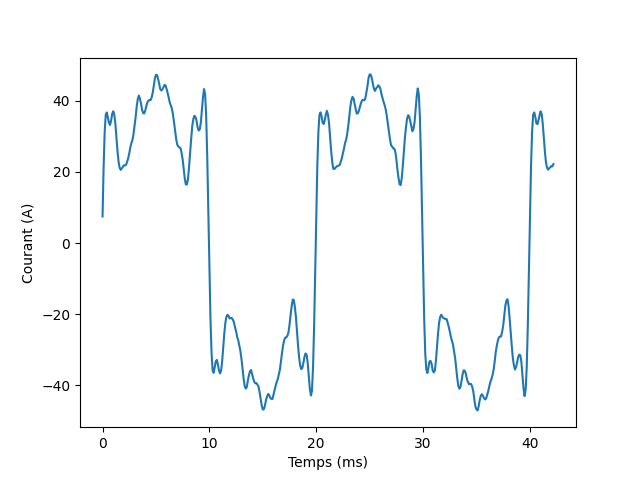
\includegraphics[width=0.92\textwidth]{simulations/courant_deforme.png}%
}
\caption{Relevé temporel du courant déformé absorbé à la menuiserie (Groupe 25).}
\label{fig:courant}
\end{figure}

\noindent
L'analyse statistique directe du signal mesuré donne :
\begin{itemize}
    \item \textbf{Valeur efficace du courant ($I_{\text{eff}}$)} : $\mathbf{\ValCourantIrms\,\text{A}}$.
    \item \textbf{Valeur de crête positive maximale} : $\mathbf{\ValCourantImax\,\text{A}}$.
    \item \textbf{Valeur de crête négative minimale} : $\mathbf{\ValCourantImin\,\text{A}}$.
    \item \textbf{Facteur de crête} : $F_c = \frac{I_{\text{max}}}{I_{\text{eff}}} = \frac{\ValCourantImax}{\ValCourantIrms} \approx 1{,}41$.
\end{itemize}
On observe une distorsion nette par rapport à une sinusoïde pure, due à la présence de charges non-linéaires (onduleurs, variateurs, redresseurs). Conformément au cahier des charges, la caractérisation fréquentielle par transformée de Fourier et le dimensionnement du filtre d'harmoniques associé feront l'objet de l'étape suivante.

\section{Sources et Références}
\begin{itemize}
    \item Cahier des charges UE12 : \emph{Sauvez l'Électron d'Arbre} (2026--2027), HELMo Gramme.
    \item Annexe 1 : Consommations et équipements de la menuiserie (Groupe 25).
    \item Annexe 2 : Plan d'implantation de la menuiserie.
    \item Annexe 3 : Relevé du courant déformé (Groupe 25).
    \item Datasheets et documentations constructeurs :
    \begin{itemize}
        \item Scie à panneaux Holzmann : \url{https://www.holzmann-maschinen.at/EN/panel-saw-1412}
        \item Scie radiale triphasée DeWalt DW721KN : \url{https://www.manualslib.com/manual/1171183/Dewalt-Dw721kn.html?page=22#manual}
        \item Aspiration centralisée LTDA : \url{https://www.ltda.fr/wp-content/uploads/2019/01/Catalogue-industriel-LTDA.pdf}
        \item Scie sur table Torros TKS316PRO 400V : \url{https://www.torros.fr/be-fr/scie-a-table-pour-le-bois-o-315-mm-400v-tks316pro400v}
        \item Ponceuse à bande monophasée Scantool : \url{https://scantool.dk/fr/product_pdf/27}
        \item Scie à ruban triphasée Cormak HBS320 NOTE: PAS DE DATASHEET PDF... AUSSI C'EST UNE SCIE A METAUX PAS A BOIS: \url{https://machinepro.fr/products/scie-ruban-pour-metaux-cormak-hbs320}
    \end{itemize}
    \item Datasheet des panneaux solaires CETC Solar NES144-7-535M : \url{https://fr.enfsolar.com/pv/panel-datasheet/crystalline/52116}
\end{itemize}

\end{document}